\documentclass[12pt,a4paper]{article}
\usepackage[utf8]{inputenc}
\usepackage[T1]{fontenc}
\usepackage{amsmath}
\usepackage{amsfonts}
\usepackage[francais]{babel}
\usepackage{amssymb}
\usepackage{graphicx}
\usepackage[top=2.00cm]{geometry}
\usepackage{enumitem}
\usepackage{tikz}
\usepackage{mathtools}
\usepackage{pgfplots}
\usetikzlibrary{plotmarks}
\usepackage{bigcenter}
\usepackage{multicol}

%Modif des enumerates numeros en gras. leftmargin=*,
\setlist[enumerate]{label=\textbf{\arabic*}.}

\usepackage{titlesec}
%modif des titres de section diminuer la taille
\titleformat{\section}
  {\normalfont\fontsize{14}{15}\bfseries}{\thesection}{1em}{}
\titleformat{\subsection}
  {\normalfont\fontsize{12}{15}\bfseries}{\thesubsection}{1em}{}


\author{CHARNAY Valentin, FINOT Sylvain}
\title{Compte rendu de TP : \\ Filtre du second ordre}

\begin{document}

\maketitle
L'objectif de ce TP est d'étudier un système electronique du second ordre et en comprendre le fonctionnement et ses applications.
\section{Réponse fréquentielle d'un système du second ordre}
\begin{enumerate}
\item Module et phase de $H(j\omega)$ avec:
 $$H(j\omega) = \frac{V_s}{V_e}(j\omega) = \frac{K}{1+2z\frac{j\omega}{\omega _n}+ \left(j\frac{\omega}{\omega _n}\right)^2}$$\\
 
 $\Rightarrow \vert H(j\omega) \vert = \frac{\vert K \vert}{\vert 1+2z\frac{j\omega}{\omega _n}+ \left(j\frac{\omega}{\omega _n}\right)^2 \vert } = \frac{K}{\sqrt{\Omega}} $\\
 Avec $\Omega = \left(1+2z\frac{j\omega}{\omega _n}+ \left(j\frac{\omega}{\omega _n}\right)^2\right)\left(1-2z\frac{j\omega}{\omega _n}+ \left(j\frac{\omega}{\omega _n}\right)^2\right)$\\
 
$\Rightarrow \vert H(j\omega) \vert  =\frac{K}{\sqrt{1 + (4z -2)(\frac{\omega}{\omega_n})^2 + (\frac{\omega}{\omega_n})^4}}  $\\
Avec $arg\left(\frac{1}{1+x}\right)= - arctan(x)$\\
Soit $\phi = arg\left( H(j\omega) \right) = - arctan\left(\frac{2z\frac{\omega}{\omega_n}}{1-\frac{\omega}{\omega_n}}\right)$\\

\item Asymptote de $\vert H(j\omega) \vert$\\
\\
- Asymptote en $\omega \rightarrow 0$ :\\
$\vert H(j\omega) \vert \underset{0}{\sim} \frac{K}{\sqrt{1}} = K $\\
- Asymptote en $\omega \rightarrow \infty $ :\\
\\
$\vert H(j\omega) \vert \underset{+\infty}{\sim} \frac{K}{\sqrt{\left(\frac{\omega}{\omega_n}\right)^4}}$\\
$\Rightarrow \vert H(j\omega) \vert \underset{+\infty}{\sim} K\left( \frac{\omega_n}{\omega}\right)^2 $\\
On peut alors que $H(j\omega) \vert_{dB +\infty} = 20. log( K\left( \frac{\omega_n}{\omega}\right)^2) $\\
$\Rightarrow H(j\omega) \vert_{dB +\infty} = -40. log(K\frac{\omega}{\omega_n})$\\
\\
On a bien une pente de -40 dB/décade.
\end{enumerate}
\section{Application au filtre de Sallen Key}
\begin{enumerate}

\item a completer
\item à completer

\item Application numérique :\\
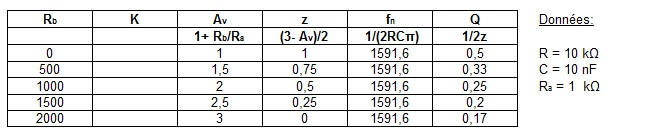
\includegraphics[scale=1]{tab1}
\end{enumerate}

\section{Excitation en régime sinusoïdal forcé}
\begin{enumerate}
\item Théoriquement, nous avons comme tension d'entrée $V_e$ = 200 mV et comme tension de sortie $V_s$ = 550 mV. Soit un gain basse fréquance $\frac{V_s}{V_e}$= 2.75\\
Expérimentalement, on mesure un gain de 2.5 ce qui est relativement proche de notre valeur théorique.

\item Fonction de transfert pour z = 0,2 \\
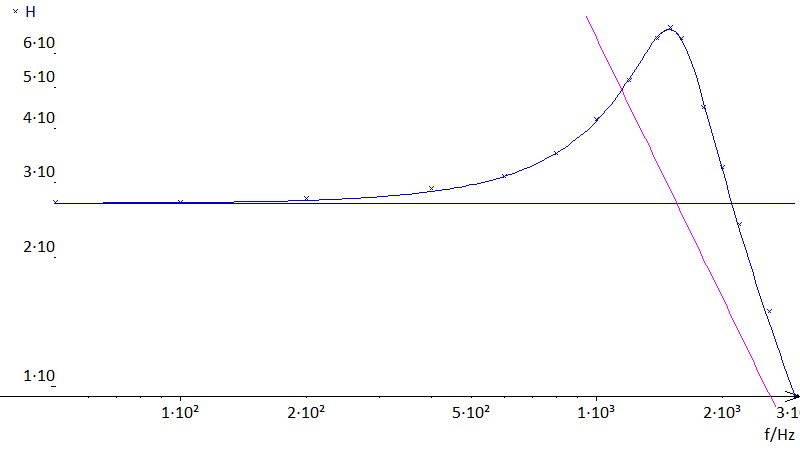
\includegraphics[scale=0.4]{graph1}
On lit alors sur le graph les valeurs de $f_n$ et ainsi $f_r$ :\\
$f_n$ = 1 560 Hz soit $f_r = f_r. \sqrt{1-2z^2}$ = 1 496 Hz \\
On observe aussi la fréquence de coupure  $f_c$ = 2 100 Hz
\end{enumerate}

\end{document}